\pr (2b) Vyberte funkciu, ktorej definičný obor je znázornený na nasledujúcom obrázku.

\begin{multicols}{2}
\scalebox{0.65}{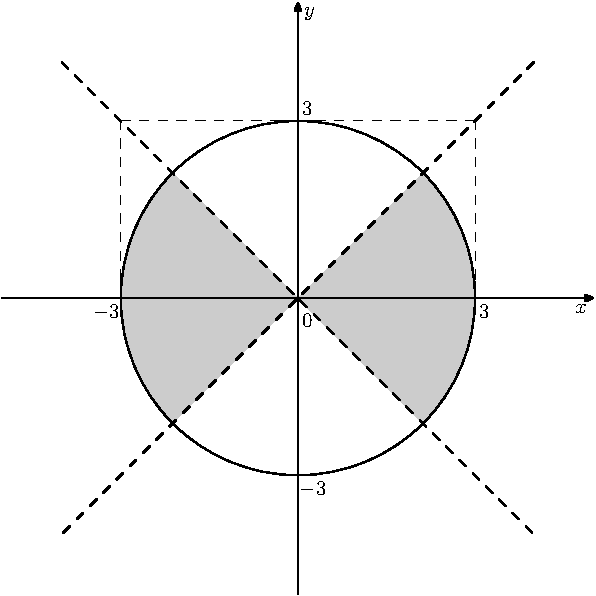
\includegraphics{Df.pdf}}

\begin{itemize}
\item[a)] $\displaystyle f(x,y)= \ln{(9-x^2-y^2)}+\ln{(x^2-y^2)}$
\item[b)] $\displaystyle f(x,y)= \sqrt{9-x^2-y^2}+\ln{(x^2-y^2)}$
\item[c)] $\displaystyle f(x,y)= \sqrt{9-x^2-y^2}+\ln{(x^2+y^2)}$
\item[d)] $\displaystyle f(x,y)= \sqrt{9-x^2-y^2}+\sqrt{x^2-y^2}$
\end{itemize}
\end{multicols}
